\documentclass[12pt]{article}

% packages :
\usepackage[utf8x]{inputenc}
\usepackage[T1]{fontenc}
%\usepackage[francais]{babel}
%
\usepackage{graphicx} % images
\usepackage{float}
\usepackage{placeins}
\usepackage{multirow}
\usepackage{wrapfig}
\usepackage{array}

% to draw circuits
\usepackage{siunitx}
\usepackage{tikz}
\usetikzlibrary{calc}
\usetikzlibrary{decorations.pathmorphing,patterns}

\usepackage[top=2cm, bottom=2cm, left=2.5cm, right=2.5cm]{geometry}


% maths :
\usepackage{amsthm}
\usepackage{amsmath}
\usepackage{amssymb}
\usepackage{mathrsfs}

\usepackage{braket}

\begin{document}

\begin{center}
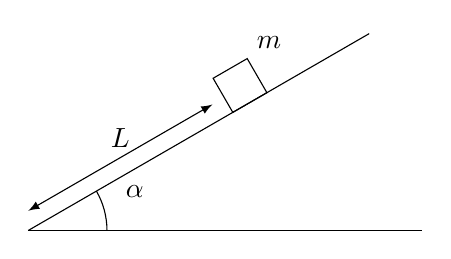
\begin{tikzpicture}
\draw (0,0) --+(5,0) ;
\draw (1,0) arc (0:30:1) node[right=.25cm]{$\alpha$};
\draw (0,0) -- +(30:5);
\draw[rotate=30] (3,0) rectangle +(.5,.5) node[anchor=south west]{$m$};
\draw[yshift=.25cm,rotate=30,latex-latex] (0,0) -- node[above]{$L$} +(2.7,0);
\end{tikzpicture}
\end{center}

\begin{center}
    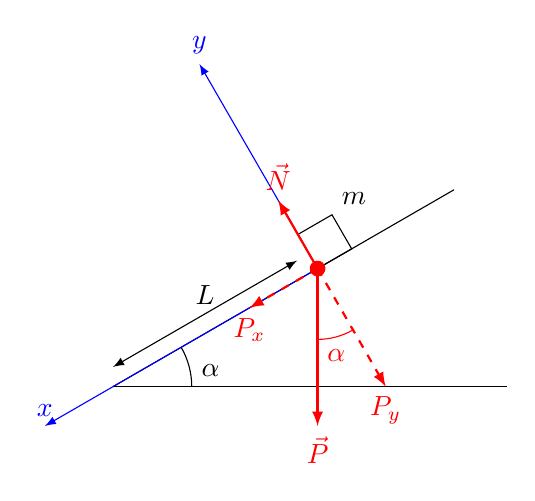
\begin{tikzpicture}
    \draw (0,0) --+(5,0) ;
    \draw (1,0) node[anchor=south west]{$\alpha$} arc (0:30:1);
    \draw (0,0) -- +(30:5);
    \draw[rotate=30] (3,0) rectangle +(.5,.5) node[anchor=south west]{$m$};
    \draw[yshift=.25cm,rotate=30,latex-latex] (0,0) -- node[above]{$L$} +(2.7,0);
    \fill[rotate=30, red] (3,0) circle (.1cm);
    \draw[rotate=30,latex-,blue] (-1,0) node[above]{$x$}-- +(4,0);
    \draw[rotate=30,-latex,blue] (3,0)-- +(0,3) node[above]{$y$};
    \draw[rotate=30,-latex,red,thick] (3,0)-- +(0,1) node[above]{$\vec{N}$};
    \draw[-latex,thick,red] (2.598,1.5) -- +(0,-2) node[below]{$\vec{P}$};
    \draw[rotate=30,-latex,red,dashed,thick] (3,0)-- +(2*-.5,0) node[below]{$P_x$};
    \draw[rotate=30,-latex,red,dashed,thick] (3,0)-- +(0,2*-0.866) node[below]{$P_y$};
    \draw[red] (2.598,1.5) -- +(0,-.9) node[anchor=north west]{$\alpha$} arc(-90:-60:.9);
    \end{tikzpicture}
\end{center}

\begin{center}
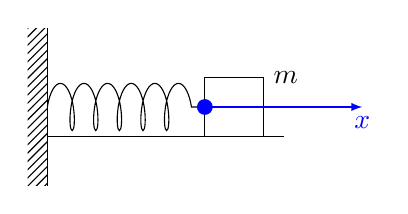
\begin{tikzpicture}
\draw (0,-1) -- +(0,2);
\fill [pattern = north east lines] (0,-1) rectangle +(-.25,2);
\draw[decoration={aspect=0.3, segment length=3mm, amplitude=3mm,coil},decorate] (0,0) -- +(2,0);
\draw (2,-.375) rectangle +(.75,.75) node[right]{$m$};
\draw (0,-.375) -- +(3,0);
\draw[blue,-latex] (2,0) -- +(2,0) node[below]{$x$}; 
\fill[blue] (2,0) circle (.1cm);
\end{tikzpicture}
\end{center}

\begin{center}
    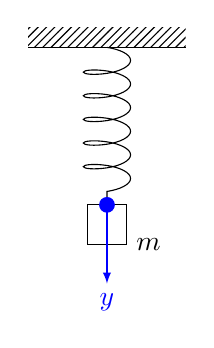
\begin{tikzpicture}
    \draw (-1,0) -- +(2,0);
    \fill [pattern = north east lines] (-1,0) rectangle +(2,.25);
    \draw[decoration={aspect=0.3, segment length=3mm, amplitude=3mm,coil},decorate] (0,0) -- +(0,-2);
    \draw (-.25,-2) rectangle +(.5,-.5) node[right]{$m$};
    \draw[blue,-latex] (0,-2) -- +(0,-1) node[below]{$y$}; 
    \fill[blue] (0,-2) circle (.1cm);
    \end{tikzpicture}
\end{center}

\begin{center}
    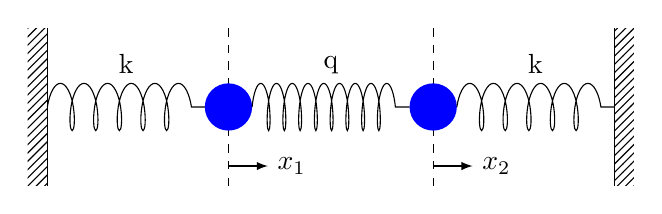
\begin{tikzpicture}
    \draw (0,-1) -- +(0,2);
    \fill [pattern = north east lines] (0,-1) rectangle +(-.25,2);
    \draw[decoration={aspect=0.3, segment length=3mm, amplitude=3mm,coil},decorate] (0,0) -- +(2,0) node[midway,above=.3cm]{k};
    \draw[dashed] (2.3,1) -- +(0,-2);
    \draw[-latex] (2.3,-.75) -- +(.5,0) node[right]{$x_1$};
    \fill[blue] (2.3,0) circle (.3cm);
    \draw[decoration={aspect=0.2, segment length=2mm, amplitude=3mm,coil},decorate] (2.6,0) -- +(2,0) node[midway,above=.3cm]{q};
    \draw[dashed] (4.9,1) -- +(0,-2);
    \draw[-latex] (4.9,-.75) -- +(.5,0) node[right]{$x_2$};
    \fill[blue] (4.9,0) circle (.3cm);
    \draw[decoration={aspect=0.3, segment length=3mm, amplitude=3mm,coil},decorate] (5.2,0) -- +(2,0) node[midway,above=.3cm]{k};
    \draw (7.2,-1) -- +(0,2);
    \fill [pattern = north east lines] (7.2,-1) rectangle +(.25,2);
    \end{tikzpicture}
\end{center}

\begin{center}
    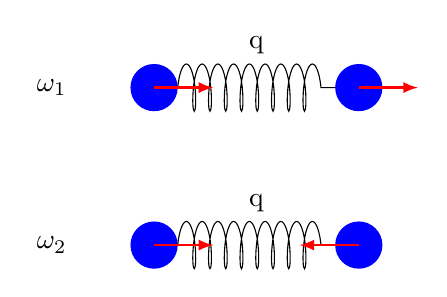
\begin{tikzpicture}
    \draw (1,0) node{$\omega_1$};
    \fill[blue] (2.3,0) circle (.3cm);
    \draw[decoration={aspect=0.2, segment length=2mm, amplitude=3mm,coil},decorate] (2.6,0) -- +(2,0) node[midway,above=.3cm]{q};
    \fill[blue] (4.9,0) circle (.3cm);
    \draw[red,thick,-latex] (2.3,0) -- +(.75,0);
    \draw[red,thick,-latex] (4.9,0) -- +(.75,0);
    
    \draw (1,-2) node{$\omega_2$};
    \fill[blue] (2.3,-2) circle (.3cm);
    \draw[decoration={aspect=0.2, segment length=2mm, amplitude=3mm,coil},decorate] (2.6,-2) -- +(2,0) node[midway,above=.3cm]{q};
    \fill[blue] (4.9,-2) circle (.3cm);
    \draw[red,thick,-latex] (2.3,-2) -- +(.75,0);
    \draw[red,thick,-latex] (4.9,-2) -- +(-.75,0);
    \end{tikzpicture}
\end{center}


\begin{center}
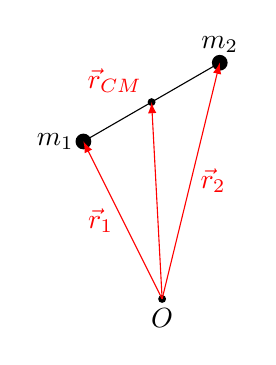
\begin{tikzpicture}
\draw (0,0) -- +(30:2);
\fill (0,0) circle (.1cm) node[left]{$m_1$};
\fill (30:2) circle (.1cm) node[above]{$m_2$};
\fill (1,-2) circle (.05cm) node[below]{$O$};
\draw[-latex,red] (1,-2) -- (0,0) node[midway,left]{$\vec{r}_1$};
\fill (30:1) circle (.05cm);
\draw[-latex,red] (1,-2) -- (30:1) node[anchor=south east]{$\vec{r}_{CM}$};
\draw[-latex,red] (1,-2) -- (30:2) node[midway,right]{$\vec{r}_2$};
\end{tikzpicture}
\end{center}

\begin{align}
i\hbar\,&\frac{\partial}{\partial t}\ket{\Psi_1(\vec{r},t)}\\
&= \hat{H}\,\ket{\Psi_1(\vec{r},t)}
\end{align}

\end{document}